\section{Managing Artists}\label{sec:managing-artists}
The \emph{Manage artists} page lists all the artists whose information has already been entered. Each artist's entry contains short information on
the number of inserted locations the artist has lived in during a period of time. These entries can be edited or deleted if necessary.

\begin{figure}[hbt!]
    \begin{center}
        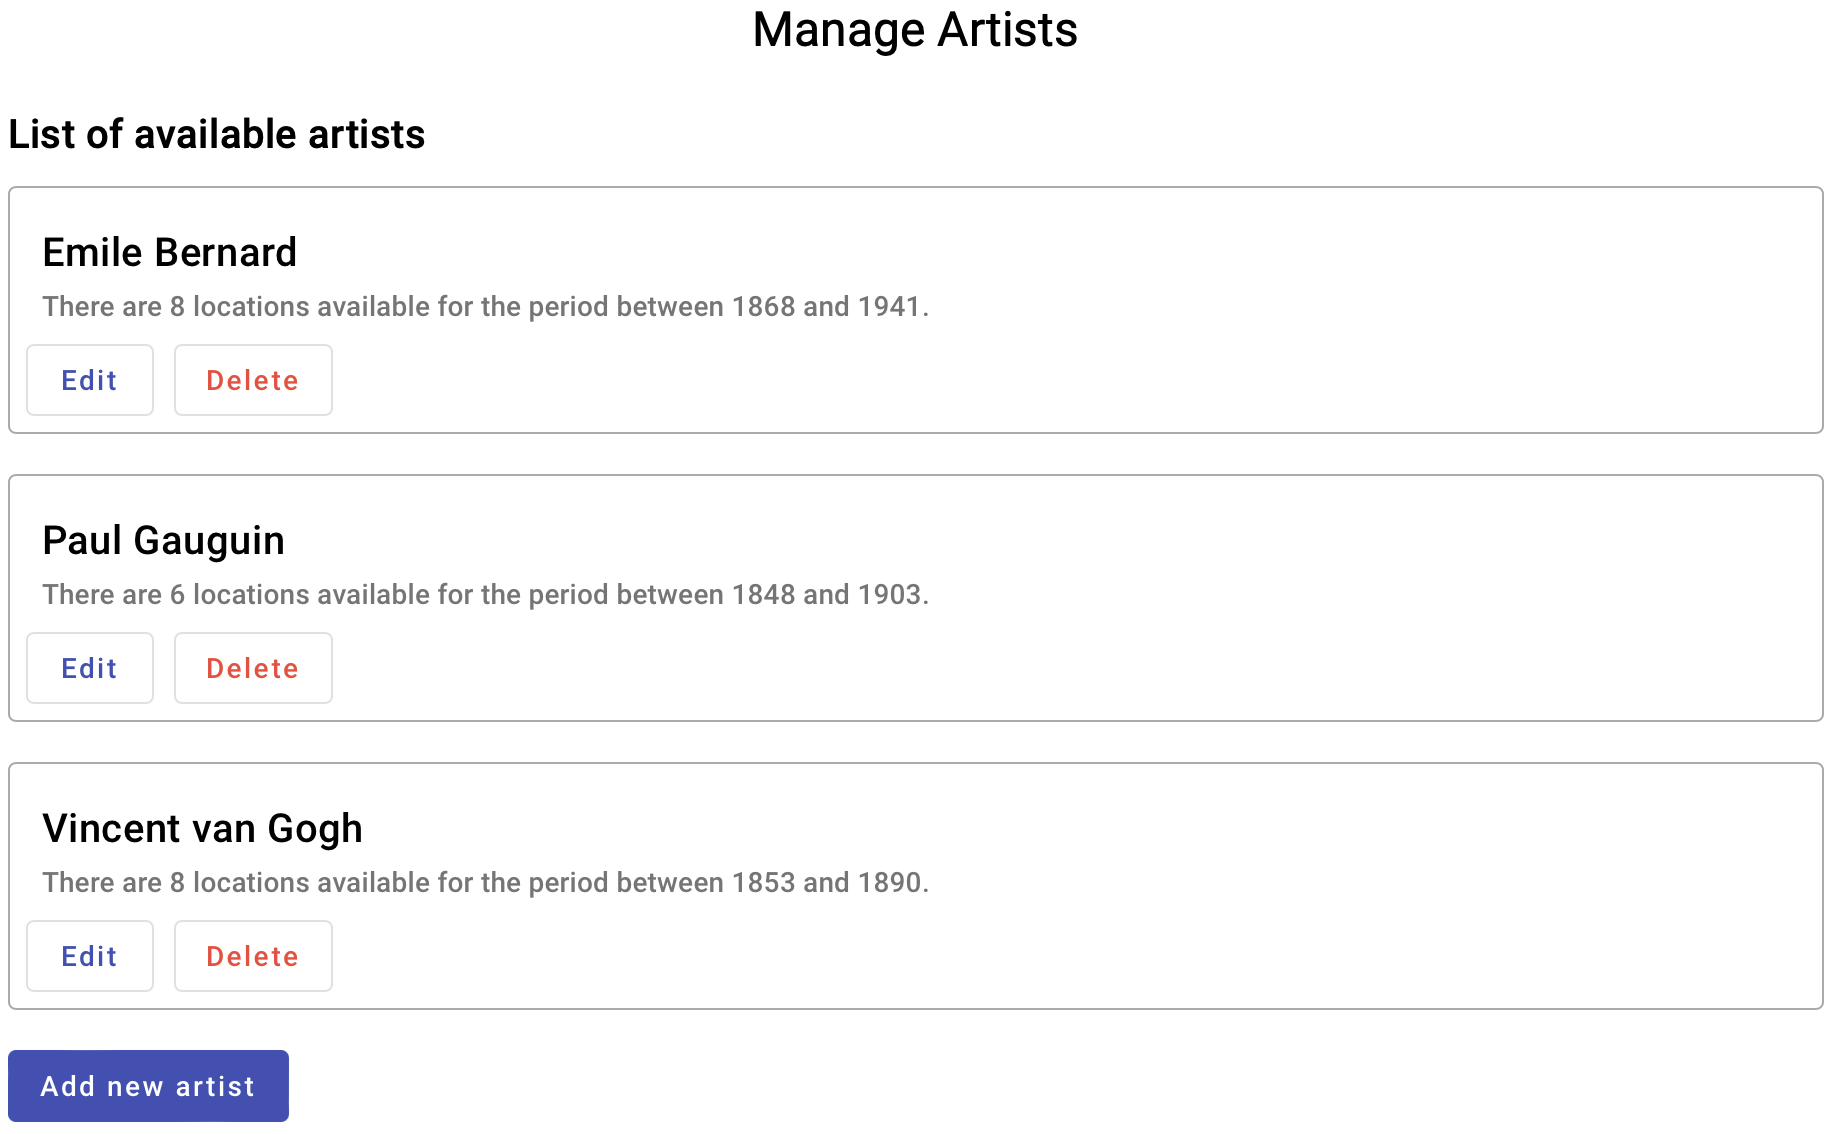
\includegraphics[width=\textwidth]{graphics/3-implementation/3}
    \end{center}
    \caption{Manage artists functionality page}
    \label{fig:figure3.3}
\end{figure}

The main functionality on this page is the addition of new artists. Selecting this option gives the user a dialog for entering all the information
related to the artists' lives, such as their name, surname, and details about the cities they lived in. Each artist’s residence includes the date
from and date until which they lived there, information related to artworks during this stay, and an option to mark the stay as important or not.
If this option is selected, a textbox appears and the user can enter a short description of why the stay was important.

\Cref{sec:impl-stc} will show how this information is presented in the cube.

\begin{figure}[hbt!]
    \begin{center}
        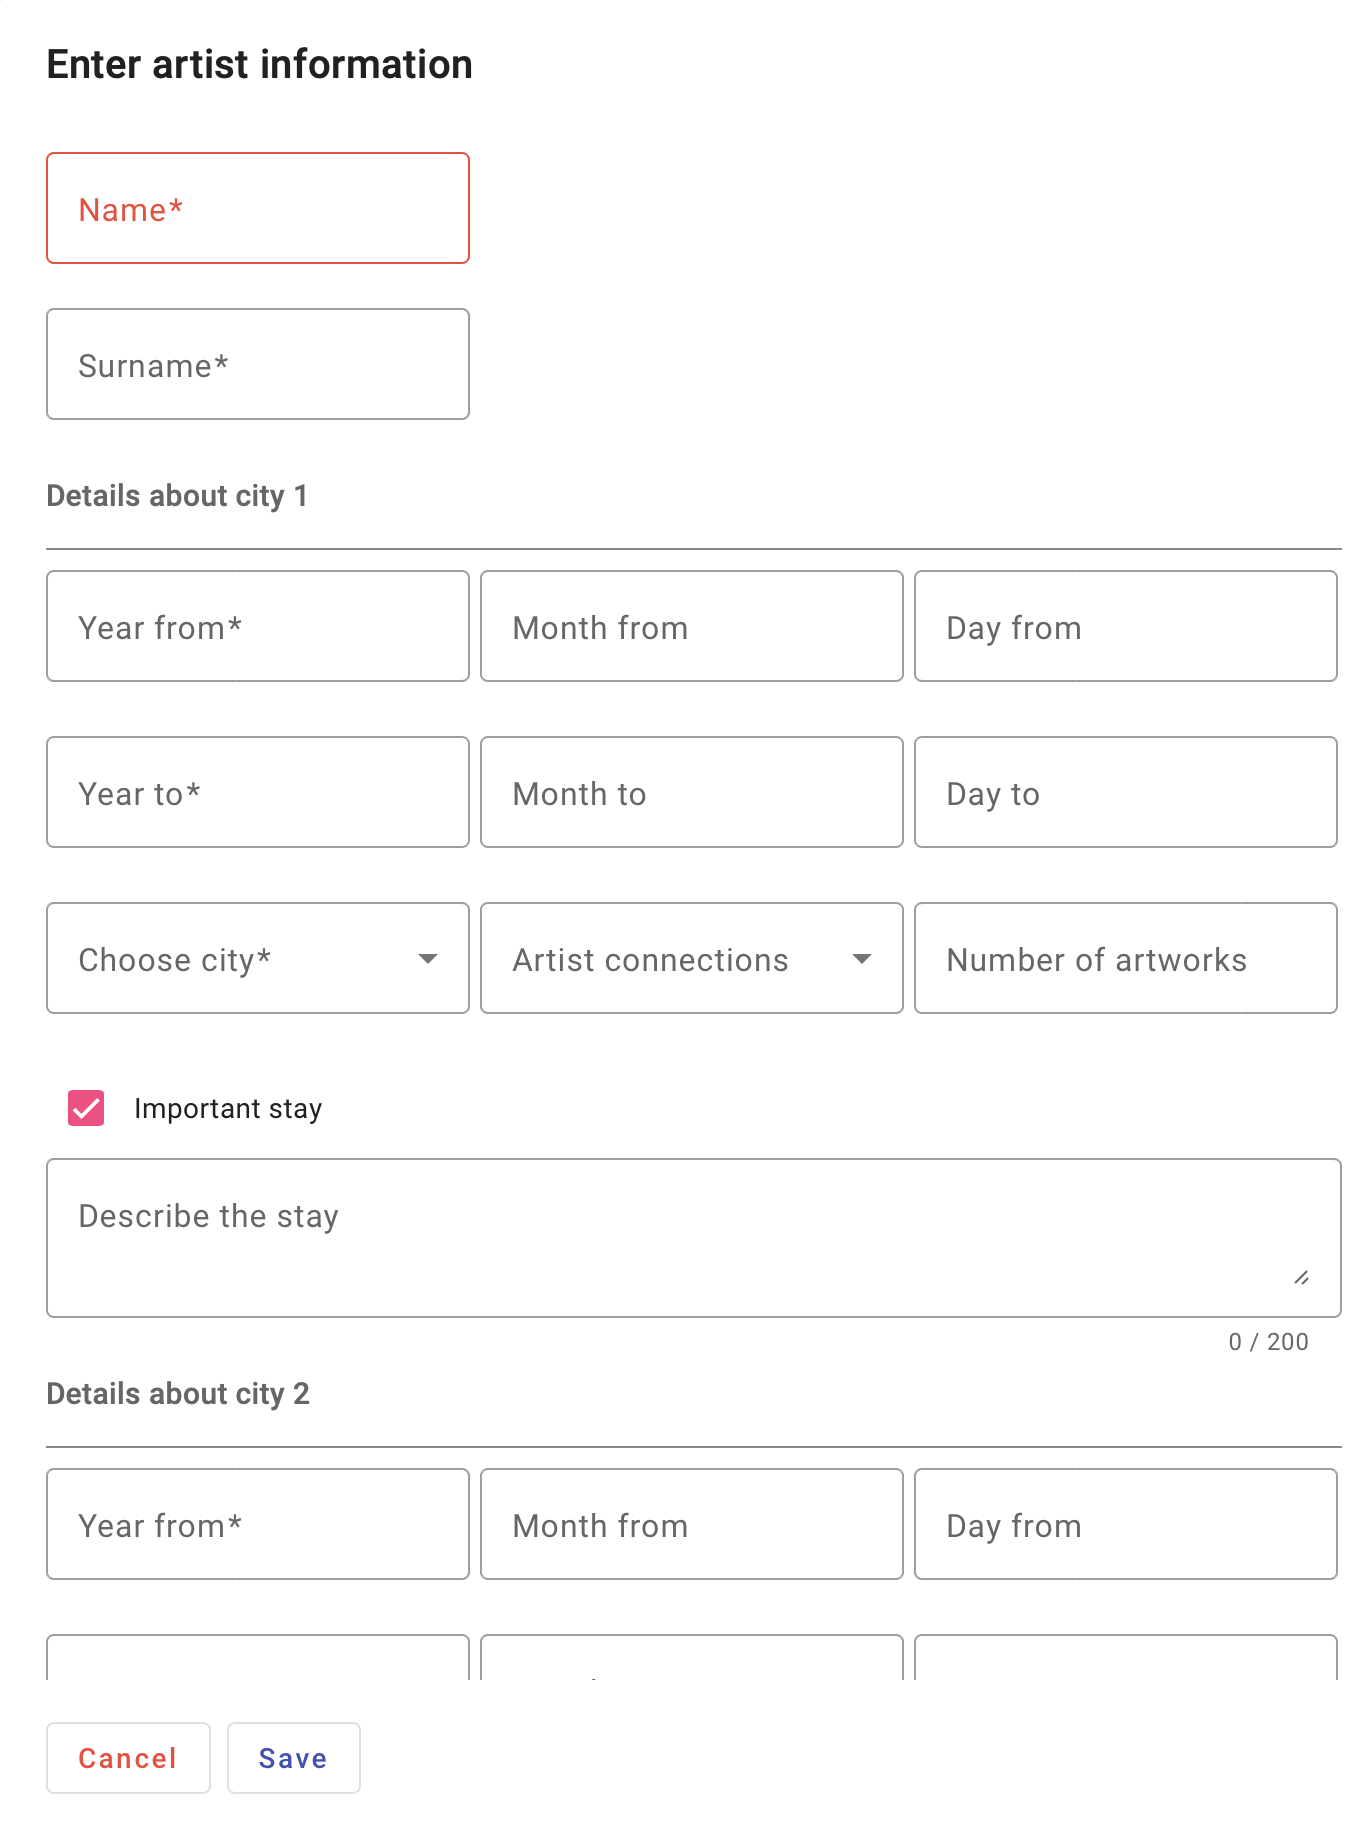
\includegraphics[width=\textwidth]{graphics/3-implementation/4}
    \end{center}
    \caption{Adding a new artist dialog}
    \label{fig:figure3.4}
\end{figure}

\clearpage